
\chapter{2. Linear PDEs: a structured grid example}

We start with the Poisson problem because it is the right place to start.  Though it is a cliche in applied mathematics, in solving it we will use key parts of \PETSc: we will build a structured grid using a \PETSc \pDMDA, then assemble a \pMat and some \pVecs in parallel on this grid, and then solve in parallel using a \pKSP object.

\section{A Poisson problem on a square domain}

The \emph{Laplacian}
    $$\grad^2 u = \Div(\grad u) = \frac{\partial^2 u}{\partial x^2} + \frac{\partial^2 u}{\partial y^2}$$
of a function $u(x,y)$ almost always appears in a mathematical model because the quantity $u$ is conserved in some sense, and because of an assumption that the gradient $\grad u$ is, up to a coefficient, the flux of $u$ \citep{Ockendonetal2003}.  The divergence ``$\Div$'' factor arises from a connection between a flux integral over a closed surface and an integral over the interior of that surface, namely the divergence (Gauss-Green) theorem \citep[Appendix C]{Evans}.

Let $\mathcal{S}$ be the open unit square $(0,1)\times(0,1)$ and denote its boundary by ``$\partial\mathcal{S}$;'' this set is simply the union of four (closed) line segments.  The following is our \emph{Poisson problem} for this Chapter;  see Figure \ref{fig:unitsquare}:
\begin{marginfigure}
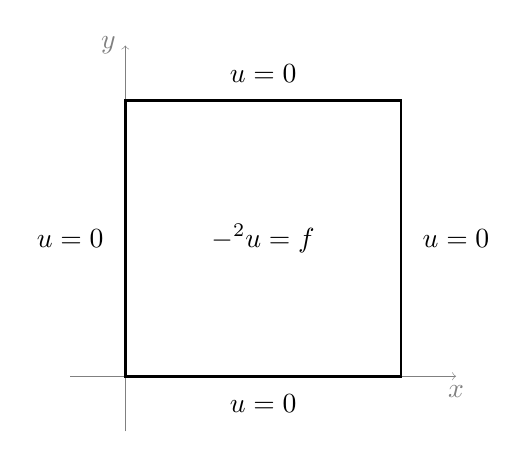
\begin{tikzpicture}[scale=3.5]
  \draw[->,gray,very thin] (-0.2,0.0) -- (1.2,0.0) node[below] {$x$};
  \draw[->,gray,very thin] (0.0,-0.2) -- (0.0,1.2) node[left] {$y$};
  \draw[line width=1.0pt] (0.0,0.0) -- (0.0,1.0) -- (1.0,1.0) -- (1.0,0.0) -- cycle;
  \node at (0.5,0.5) {$- \grad^2 u = f$};
  \node at (0.5,-0.1) {$u = 0$};
  \node at (0.5,1.1) {$u = 0$};
  \node at (-0.2,0.5) {$u = 0$};
  \node at (1.2,0.5) {$u = 0$};
\end{tikzpicture}
\caption{Our first, simple goal is to solve the Poisson equation on the unit square $\mathcal{S}$, with homogeneous Dirichlet boundary conditions.}
\label{fig:unitsquare}
\end{marginfigure}
\begin{align}
- \grad^2 u &= f \quad \text{ on } \mathcal{S}, \label{poissonsquare} \\
u &= 0 \quad \text{ on } \partial \mathcal{S}. \notag
\end{align}
The PDE in \eqref{poissonsquare} is the \emph{Poisson equation}.  We will not just solve this one equation on a finite region, however.  The boundary conditions in \eqref{poissonsquare}, where $u$ is set to zero along the boundary of $\mathcal{S}$, are called ``\emph{homogeneous Dirichlet}.''  Historically the problem \eqref{poissonsquare} is more properly called the \emph{Dirichlet problem}, but we call it the Poisson problem because we will think about it flexibly, with various boundary conditions (e.g.~in Chapter 3).  The whole problem must include boundary conditions, either Dirichlet ($u$ known) or Neumann (derivative of $u$ known) or a combination, and then we will expect it to determine a solution.  We will approximate that solution numerically.

The Poisson problem can model the electrostatic potential, the equilibrium distribution from certain random walks, the distribution of temperature in a conducting object at steady state, and many other other physical phenomena.  For example, in the context of heat conduction Fourier's law says $\bq = -k \grad u$, where $k$ is approximately constant if the variation in $u$ is not too large.  Conservation of energy for a solid says $c\rho \partial u/\partial t = - \Div\bq + f$ if $f$ describes a heat source within the domain.  At steady state these facts combine to give $0 = k \grad^2 u + f$, that is, Poisson's equation \eqref{poissonsquare}.  Holding the temperature fixed at zero along the boundary completes the problem.

For this chapter we will suppose that $f(x,y)$ is continuous and bounded on $\mathcal{S}$, so that we can compute its pointwise values.  With our homogeneous Dirichlet boundary conditions, and the assumptions on $f$, standard theory says that $u(x,y)$ exists and is continuous on the closed square $\overline{\mathcal{S}}$ \citep[Theorem 6 in section 5.6]{Evans}.\sidenote{A classical approach to showing existence starts by solving problem \eqref{poissonsquare} by Fourier series.  If $f$ is square-integrable then the coefficients $\hat f$ are square-integrable (Parseval's equality).  Because the Laplacian is elliptic and second-order, the coefficients $\hat u$ are square-integrable even when multiplied by the frequency squared.  By Cauchy-Schwarz, the Fourier series for $u$ is the limit of a sequence of continuous functions on $\overline{\mathcal{S}}$ which converge uniformly, so $u\in C^0(\overline{\mathcal{S}})$.}  Thus there is no ambiguity in the boundary condition ``$u=0$ on $\partial \mathcal{S}$,'' and also we can sensibly discuss the pointwise values $u(x,y)$.

Without any boundary conditions, the Poisson equation $-\grad^2 u = f$ alone is not a well-posed problem because if $u$ is a solution then $v=u+C$ is also a solution for any constant $C$.  (In fact there are constant solutions $w=C$ and many, many more to the Laplace equation $-\grad^2 w = 0$ on $\mathcal{S}$.)  However, with the Dirichlet boundary conditions in \eqref{poissonsquare}, the solution is unique if it exists \citep[Theorem 5 in section 2.2]{Evans}; \citep[subsection 5.2.1]{Ockendonetal2003}.


\section{A finite difference method: build the grid}

Because \eqref{poissonsquare} is a linear problem, finite-dimensional approximations of it are simply linear systems.  The finite-dimensional approximation in this Chapter comes from applying a \emph{finite difference} (FD) method.  In Chapter 3 we will apply a finite element approach instead.

\begin{marginfigure}
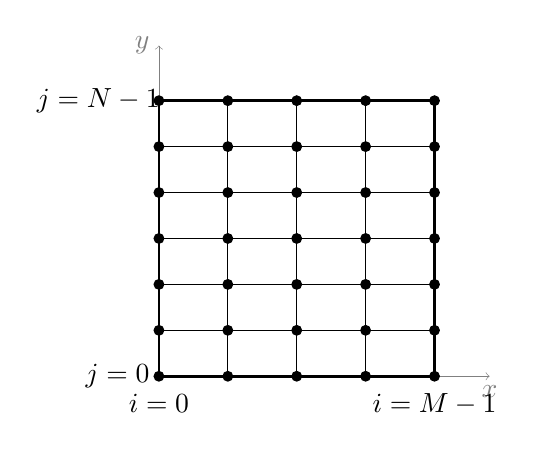
\begin{tikzpicture}[scale=3.5]
  \draw[->,gray,very thin] (0.0,0.0) -- (1.2,0.0) node[below] {$x$};
  \draw[->,gray,very thin] (0.0,0.0) -- (0.0,1.2) node[left] {$y$};
  \draw[line width=1.0pt] (0.0,0.0) -- (0.0,1.0) -- (1.0,1.0) -- (1.0,0.0) -- cycle;
  \node at (0.0,-0.1) {$i=0$};
  \node at (1.0,-0.1) {$i=M-1$};
  \node at (-0.15,0.0) {$j=0$};
  \node at (-0.22,1.0) {$j=N-1$};
  \pgfmathsetmacro\fourth{1.0/4.0}
  \pgfmathsetmacro\sixth{1.0/6.0}
  \draw[xstep=\fourth,ystep=\sixth,black,thin] (0.0,0.0) grid (1.0,1.0);
  \foreach \x in {0,...,4} {
    \foreach \y in {0,...,6} {
        \filldraw (\x * \fourth,\y * \sixth) circle (0.5pt);
    }
  }
\end{tikzpicture}
\caption{A grid on the unit square $\mathcal{S}$, with $M=5$ and $N=7$.}
\label{fig:unitsquaregrid}
\end{marginfigure}

To start our FD method we put a \emph{structured grid} of $MN$ points on the unit square, as in Figure \ref{fig:unitsquaregrid}, with spacing $h_x=1/(M-1)$ and $h_y=1/(N-1)$ in the two directions.  The grid coordinates are $x_i = i\, h_x$ for $i = 0,1,\dots,M-1$ and $y_j = j\, h_y$ and $j=0,1,\dots,N-1$.

The construction of such a two-dimensional (2D) grid, and the distribution of it across processors, will be our first new idea from \PETSc, beyond the basics in Chapter 1.  Consider the lines of code in Figure \ref{code:dmdacreatetwod}.  They create a \PETSc \pDM object\sidenote{``\pDM'' might stand for ``data management'', but perhaps ``distributed mesh'' is better.} for a grid like Figure \ref{fig:unitsquaregrid}.

\clearpage
\cinputraw{dmdacreate2d.frag}{extract from c2poisson.c}{An example of creating a 2D \pDMDA.}{}{//START}{//STOP}{code:dmdacreatetwod}

A \pDM is an abstract type for describing the topology (i.e.~connectedness) of a grid, \emph{and} the way it is distributed across \MPI processes, \emph{and} the way each process can access data from its neighbors.  The specific variable \texttt{da} in Figure \ref{code:dmdacreatetwod} has type ``\pDMDA'', which is the subclass of \pDM s which are structured grids.

The Figure \ref{code:dmdacreatetwod} code is a part of \texttt{c2poisson.c} below, which solves Poisson's problem.  Thus, if we do
\begin{Verbatim}[fontsize=\small]
  make c2poisson
  ./c2poisson -da_grid_x 5 -da_grid_y 7
\end{Verbatim}
then a structured grid will be created which is exactly as shown in Figure \ref{fig:unitsquaregrid}.  In this case all points of the grid are ``owned'' by the single created when we run \texttt{c2poisson} without \MPI.

\begin{marginfigure}
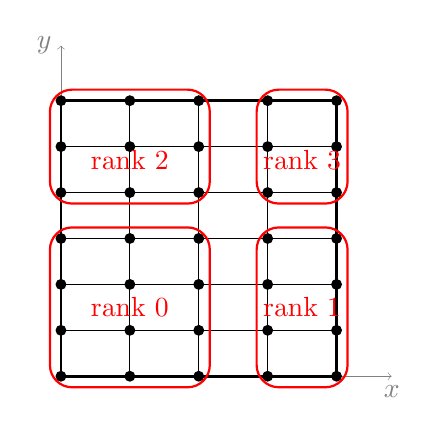
\begin{tikzpicture}[scale=3.5]
  \draw[->,gray,very thin] (0.0,0.0) -- (1.2,0.0) node[below] {$x$};
  \draw[->,gray,very thin] (0.0,0.0) -- (0.0,1.2) node[left] {$y$};
  \draw[line width=1.0pt] (0.0,0.0) -- (0.0,1.0) -- (1.0,1.0) -- (1.0,0.0) -- cycle;
  \pgfmathsetmacro\fourth{1.0/4.0}
  \pgfmathsetmacro\sixth{1.0/6.0}
  \draw[xstep=\fourth,ystep=\sixth,black,thin] (0.0,0.0) grid (1.0,1.0);
  \foreach \x in {0,...,4} {
    \foreach \y in {0,...,6} {
        \filldraw (\x * \fourth,\y * \sixth) circle (0.5pt);
    }
  }
  \pgfmathsetmacro\dd{0.04}
  \pgfmathsetmacro\od{1.04}
  \pgfmathsetmacro\xap{2*\fourth + 0.04}
  \pgfmathsetmacro\xbm{3*\fourth - 0.04}
  \pgfmathsetmacro\yap{3*\sixth + 0.04}
  \pgfmathsetmacro\ybm{4*\sixth - 0.04}
  \pgfmathsetmacro\xamid{1*\fourth}
  \pgfmathsetmacro\xbmid{3.5*\fourth}
  \pgfmathsetmacro\yamid{1.5*\sixth}
  \pgfmathsetmacro\ybmid{4.7*\sixth}
  \draw[thick,rounded corners=8pt,color=red]
    (-\dd,-\dd) -- (-\dd,\yap) -- (\xap,\yap) -- (\xap,-\dd) -- cycle;
  \node[color=red] at (\xamid,\yamid) {rank $0$};
  \draw[thick,rounded corners=8pt,color=red]
    (\xbm,-\dd) -- (\od,-\dd) -- (\od,\yap) -- (\xbm,\yap) -- cycle;
  \node[color=red] at (\xbmid,\yamid) {rank $1$};
  \draw[thick,rounded corners=8pt,color=red]
    (-\dd,\ybm) -- (\xap,\ybm) -- (\xap,\od) -- (-\dd,\od) -- cycle;
  \node[color=red] at (\xamid,\ybmid) {rank $2$};
  \draw[thick,rounded corners=8pt,color=red]
    (\xbm,\ybm) -- (\od,\ybm) -- (\od,\od) -- (\xbm,\od) -- cycle;
  \node[color=red] at (\xbmid,\ybmid) {rank $3$};
\end{tikzpicture}
\caption{The same grid as in Figure \ref{fig:unitsquaregrid}, distributed across four \MPI processes (i.e.~with \texttt{rank} $\in \{0,1,2,3\}$) automatically by \texttt{DMDACreate2d()}.}
\label{fig:unitsquaregridparallel}
\end{marginfigure}

However, if we run it with multiple \MPI processes by
\begin{Verbatim}[fontsize=\small]
  mpiexec -n N ./c2poisson -da_grid_x Mx -da_grid_y My
\end{Verbatim}
then \PETSc does the best it can to balance the load of \texttt{Mx}$\cdot$\texttt{My} grid points among \texttt{N} processes, with the restriction that each \MPI process owns a rectangular subgrid when we use a \pDMDA object to manage the grid.  For example, if we do
\begin{Verbatim}[fontsize=\small]
  mpiexec -n 4 ./c2poisson -da_grid_x 5 -da_grid_y 7
\end{Verbatim}
then the distributed structured grid shown in Figure \ref{fig:unitsquaregridparallel} will be created.  Neither \texttt{Mx}$=5$ nor \texttt{My}$=7$ is divisible by two, but \PETSc distributes the four ranks across the \texttt{Mx}$\cdot$\texttt{My}$=35$ nodes (grid points) relatively uniformly: the rank $0$ process owns 12 grid points and the rank $3$ process owns 6, while the other ranks are in between.  In this case the load is only balanced to within a factor of two, but larger grids will be better load-balanced.  

\begin{marginfigure}
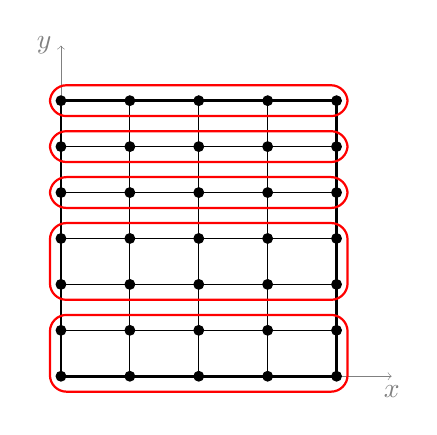
\begin{tikzpicture}[scale=3.5]
  \draw[->,gray,very thin] (0.0,0.0) -- (1.2,0.0) node[below] {$x$};
  \draw[->,gray,very thin] (0.0,0.0) -- (0.0,1.2) node[left] {$y$};
  \draw[line width=1.0pt] (0.0,0.0) -- (0.0,1.0) -- (1.0,1.0) -- (1.0,0.0) -- cycle;
  \pgfmathsetmacro\fourth{1.0/4.0}
  \pgfmathsetmacro\sixth{1.0/6.0}
  \draw[xstep=\fourth,ystep=\sixth,black,thin] (0.0,0.0) grid (1.0,1.0);
  \foreach \x in {0,...,4} {
    \foreach \y in {0,...,6} {
        \filldraw (\x * \fourth,\y * \sixth) circle (0.5pt);
    }
  }
  \pgfmathsetmacro\dd{0.04}
  \pgfmathsetmacro\od{1.04}
  \foreach \y in {0,2} {
    \pgfmathsetmacro\yup{\y * \sixth - 1.4 * \dd}  % less than 1.7 generates flaw?
    \pgfmathsetmacro\ydn{(\y + 1) * \sixth + 1.4 * \dd}
    \draw[thick,rounded corners=6pt,color=red]
      (-\dd,\ydn) -- (\od,\ydn) -- (\od,\yup) -- (-\dd,\yup) -- cycle;
  }
  \foreach \y in {4,5,6} {
    \pgfmathsetmacro\yup{\y * \sixth - 1.4 * \dd}  % less than 1.7 generates flaw?
    \pgfmathsetmacro\ydn{\y * \sixth + 1.4 * \dd}
    \draw[thick,rounded corners=6pt,color=red]
      (-\dd,\ydn) -- (\od,\ydn) -- (\od,\yup) -- (-\dd,\yup) -- cycle;
  }
\end{tikzpicture}
\caption{Processor domains are far from square if the total number of \MPI processes is prime, because only one dimension can be decomposed.  We show what \texttt{-dm\_view} reports for the same grid as in Figure \ref{fig:unitsquaregrid}, with \texttt{mpiexec -n 5}.}
\label{fig:unitsquaregridprime}
\end{marginfigure}

The fifth and sixth arguments ``\texttt{-10}'' to \texttt{DMDACreate2d()} in Figure \ref{code:dmdacreatetwod} are used to set default dimensions $M=10$ and $N=10$.  We have seen that these defaults are overridden by runtime options \texttt{-da\_grid\_x} and \texttt{-da\_grid\_y}.  However, if we do this,
 \begin{Verbatim}[fontsize=\small]
  mpiexec -n 4 ./c2poisson
\end{Verbatim}
then a structured grid will be distributed across the four processes as in Figure \ref{fig:unitsquaregrideight}, with each rank owning 25 nodes.  \PETSc itself can show the parallel layout by calling
\begin{Verbatim}[fontsize=\small]
  mpiexec -n 4 ./c2poisson -dm_view
\end{Verbatim}
or
\begin{Verbatim}[fontsize=\small]
  mpiexec -n 4 ./c2poisson -dm_view draw -draw_pause 2
\end{Verbatim}
The latter version shows the grid graphically, for two seconds.

\begin{marginfigure}
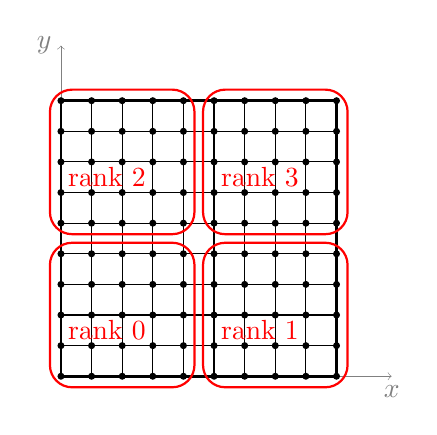
\begin{tikzpicture}[scale=3.5]
  \draw[->,gray,very thin] (0.0,0.0) -- (1.2,0.0) node[below] {$x$};
  \draw[->,gray,very thin] (0.0,0.0) -- (0.0,1.2) node[left] {$y$};
  \draw[line width=1.0pt] (0.0,0.0) -- (0.0,1.0) -- (1.0,1.0) -- (1.0,0.0) -- cycle;
  \pgfmathsetmacro\ninth{1.0/9.0}
  \draw[xstep=\ninth,ystep=\ninth,black,thin] (0.0,0.0) grid (1.0,1.0);
  \foreach \x in {0,...,9} {
    \foreach \y in {0,...,9} {
        \filldraw (\x * \ninth,\y * \ninth) circle (0.3pt);
    }
  }
  \pgfmathsetmacro\dd{0.04}
  \pgfmathsetmacro\od{1.04}
  \pgfmathsetmacro\ap{4*\ninth + 0.04}
  \pgfmathsetmacro\bm{5*\ninth - 0.04}
  \pgfmathsetmacro\amid{1.5*\ninth}
  \pgfmathsetmacro\bmid{6.5*\ninth}
  \draw[thick,rounded corners=8pt,color=red]
    (-\dd,-\dd) -- (-\dd,\ap) -- (\ap,\ap) -- (\ap,-\dd) -- cycle;
  \node[color=red] at (\amid,\amid) {rank $0$};
  \draw[thick,rounded corners=8pt,color=red]
    (\bm,-\dd) -- (\od,-\dd) -- (\od,\ap) -- (\bm,\ap) -- cycle;
  \node[color=red] at (\bmid,\amid) {rank $1$};
  \draw[thick,rounded corners=8pt,color=red]
    (-\dd,\bm) -- (\ap,\bm) -- (\ap,\od) -- (-\dd,\od) -- cycle;
  \node[color=red] at (\amid,\bmid) {rank $2$};
  \draw[thick,rounded corners=8pt,color=red]
    (\bm,\bm) -- (\od,\bm) -- (\od,\od) -- (\bm,\od) -- cycle;
  \node[color=red] at (\bmid,\bmid) {rank $3$};
\end{tikzpicture}
\caption{An $M=10$ by $N=10$ grid distributed by \texttt{DMDACreate2d()} across four \MPI processes.}
\label{fig:unitsquaregrideight}
\end{marginfigure}

To explain the other options to \texttt{DMDACreate2d()} we start by quoting the \PETSc manual pages description:

\noindent\hrulefill
\begin{Verbatim}[fontsize=\small]
DMDACreate2d(MPI_Comm comm, DMBoundaryType bx, DMBoundaryType by,
  DMDAStencilType stype, PetscInt M, PetscInt N, PetscInt m, PetscInt n,
  PetscInt dof, PetscInt s, const PetscInt lx[], const PetscInt ly[],
  DM *da)
\end{Verbatim}
where
\small
\begin{itemize}[align=left]
\item[\texttt{comm}]   MPI communicator \\
\item[\texttt{bx,by}]  type of ghost nodes the array have; use one of \texttt{DM\_BOUNDARY\_NONE, DM\_BOUNDARY\_GHOSTED, DM\_BOUNDARY\_PERIODIC} \\
\item[\texttt{stype}] stencil type; use either \texttt{DMDA\_STENCIL\_BOX} or \texttt{DMDA\_STENCIL\_STAR} \\
\item[\texttt{M,N}]	   global dimension in each direction of the array; use \texttt{-M} and or \texttt{-N} to indicate that it may be set to a different value from the command line with \texttt{-da\_grid\_x <M> -da\_grid\_y <N>} \\
\item[\texttt{m,n}]   corresponding number of processors in each dimension (or \texttt{PETSC\_DECIDE} to have calculated) \\
\item[\texttt{dof}]     number of degrees of freedom per node \\
\item[\texttt{s}]       stencil width \\
\item[\texttt{lx,ly}]  arrays containing the number of nodes in each cell along the x and y coordinates, or \texttt{NULL}; if non-null, these must be of length as m and n, and the corresponding m and n cannot be \texttt{PETSC\_DECIDE}; the sum of the \texttt{lx[]} entries must be M, and the sum of the \texttt{ly[]} entries must be N \\
\item[\texttt{da}]      output: the resulting distributed array object 
\end{itemize}
\normalsize
\noindent\hrulefill
\medskip

\noindent In Figure \ref{code:dmdacreatetwod}, the first argument to \texttt{DMDACreate2d()} is a serial or parallel \MPI communicator.  In the second and third arguments we have used ``\texttt{DM\_BOUNDARY\_NONE}'' because our Dirichlet boundary condition does not require communication to the next process' domain, nor periodic wrapping.  In the fourth argument we use \texttt{DMDA\_STENCIL\_STAR} because only cardinal neighbors of a grid point are used when forming the matrix; we will address the FD ``stencil'' below.  As already noted, the fifth and sixth arguments set $M=10,N=10$ as override-able grid defaults.  In the next two arguments, ``\texttt{PETSC\_DECIDE}'' tells \PETSc to decompose our grid over \MPI processes according to the size of (i.e.~number of processes in) the \MPI communicator and its internal logic, as described above.  The next two arguments, in the ninth and tenth positions, say that our PDE is scalar (\texttt{dof}$=1$) and that the FD method only needs one neighbor in each \texttt{STENCIL\_STAR} direction (\texttt{s}$=1$).  The next two arguments are \texttt{NULL} because we are \emph{not} telling \PETSc any details about how to distribute processes over the grid; it \texttt{DECIDE}s for itself.  Finally, the \pDMDA object is created as an output.

The call to \texttt{DMDASetUniformCoordinates()} in Figure \ref{code:dmdacreatetwod} sets the domain to be $[0,1]\times[0,1]$.  The last two arguments are ignored in this case; they would set limits on the third dimension if \texttt{da} was created with \texttt{DMDACreate3d()}.

To wrap up our coverage of creating distributed grids, the standard \PETSc view of what \pDM s ``look like'' is in Figure \ref{fig:petscghostvalues}.  On the left is a version of what we have done in the code in Figure \ref{code:dmdacreatetwod}, namely create a structured grid \pDM.  The one shown in Figure \ref{fig:petscghostvalues} has \texttt{DMDA\_STENCIL\_BOX} stencil type, unlike ours.  On the right is an unstructured grid, of the type created in Chapter 3 for the finite element method.  In both cases the figure shows nodes owned by a given process (red ``local'' nodes) and those other nodes that are accessible by the local process (blue ``ghost'' nodes).  We will see such local/ghost node types in all examples in this book, and address their role again in future examples.

\begin{figure}
\includegraphics[width=\textwidth]{petscghostvalues}
\caption{\PETSc's parallel decomposition of structured and unstructured grids, showing owned (``local'') and accessible (``ghost'') nodes for one process.}
\label{fig:petscghostvalues}
\end{figure}


\section{A finite difference method: assemble the linear system}

Recall we were trying to approximate PDE problem \eqref{poissonsquare}.  Having built a structured grid we can now return to the FD method.

By a well-known Taylor's theorem argument \citep{MortonMayers}, for any function $F(x)$ which is sufficiently smooth, we have
    $$F''(x) = \frac{F(x+h) - 2 F(x) + F(x-h)}{h^2} + O(h^2)$$
as $h$ goes to zero.  This formula, applied to partial derivatives, will give an approximation of the Laplacian in problem \eqref{poissonsquare}.

Let $U_{i,j}$ be the gridded approximation to the exact value $u(x_i,y_j)$ of the solution at a grid point,\sidenote{This is an important sentence!  We \emph{compute} values $U_{i,j}$ from the finite difference equations.  We generally \emph{don't know} the values $u(x_i,y_j)$.  Of course we want the former to be close to the latter.}  and also denote $f_{i,j} = f(x_i,y_j)$.  Then we have this FD approximation to problem \eqref{poissonsquare}:
\begin{equation}
- \frac{U_{i+1,j} - 2 U_{i,j} + U_{i-1,j}}{h_x^2} - \frac{U_{i,j+1} - 2 U_{i,j} + U_{i,j-1}}{h_y^2} = f_{i,j}. \label{poissonsquareFDearly}
\end{equation}
Equation \eqref{poissonsquareFDearly} applies for all of the interior points where $1 \le i \le M-2$ and $1 \le j \le N-2$.  The boundary conditions in \eqref{poissonsquare} become
\begin{equation}
U_{0,j} = 0, \quad U_{M-1,j} = 0, \quad U_{i,0} = 0, \quad U_{i,N-1} = 0, \label{poissonsquareFDbcs}
\end{equation}
for all $i,j$.

At a grid location $(x_i,y_j)$, equation \eqref{poissonsquareFDearly} relates the unknown $U_{i,j}$ to its four cardinal neighbors $U_{i+1,j}$, $U_{i-1,j}$, $U_{i,j+1}$, and $U_{i,j-1}$.  This pattern is a \emph{stencil}, in particular a ``star'' stencil, as shown in Figure \ref{fig:unitsquaregridstencil}.  A ``box'' stencil would also involve all the diagonal neighbors.  In 2D, an equation using a star stencil relates at most five unknowns, while one with a box stencil relates at most nine unknowns.

\begin{marginfigure}
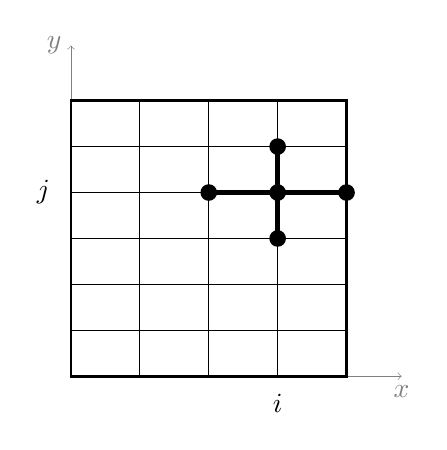
\begin{tikzpicture}[scale=3.5]
  \draw[->,gray,very thin] (0.0,0.0) -- (1.2,0.0) node[below] {$x$};
  \draw[->,gray,very thin] (0.0,0.0) -- (0.0,1.2) node[left] {$y$};
  \draw[line width=1.0pt] (0.0,0.0) -- (0.0,1.0) -- (1.0,1.0) -- (1.0,0.0) -- cycle;
  \node at (0.75,-0.1) {$i$};
  \node at (-0.1,0.666667) {$j$};
  \filldraw (0.50,0.666667) circle (0.8pt);
  \filldraw (0.75,0.666667) circle (0.8pt);
  \filldraw (1.00,0.666667) circle (0.8pt);
  \filldraw (0.75,0.5) circle (0.8pt);
  \filldraw (0.75,0.833333) circle (0.8pt);
  \draw[line width=2.0pt] (0.50,0.666667) -- (1.00,0.666667);
  \draw[line width=2.0pt] (0.75,0.5)  -- (0.75,0.833333);
  \draw[xstep=0.25,ystep=0.166667,black,thin] (0.0,0.0) grid (1.0,1.0);
\end{tikzpicture}
\caption{A ``star'' stencil, shown on the same grid as in Figure \ref{fig:unitsquaregrid}, at $i=3$ and $j=4$.}
\label{fig:unitsquaregridstencil}
\end{marginfigure}

Equations \eqref{poissonsquareFDearly} and \eqref{poissonsquareFDbcs} form a linear system of $K=MN$ equations in which we choose to treat all values $U_{i,j}$ on the grid, whether on the boundary or in the interior, as unknowns.  To shown this linear system in traditional form
\begin{equation}
A \bu = \bb, \label{poissonlinearsystem}
\end{equation}
where $A$ is a $K\times K$ matrix and $\bu,\bb$ are $K\times 1$ column vectors, we must order the unknowns.  Such an ordering is implemented inside a \PETSc \pDMDA.  We use it here for displaying the system, but the code we actually write uses the grid-wise coordinates $(i,j)$.

The ordering used in serial in a 2D \pDMDA is shown in the $M=4$ and $N=3$ case in Figure \ref{fig:unitsquaregridordering}.  One could write this ordering as
\begin{equation}
    U_k = U_{i,j} \quad \text{ where } \quad k = j\,M + i. \label{orderingfd}
\end{equation}
We will let \PETSc do such index transformations internally inside the \pDMDA implementation.  However, now is a good time to also show the linear system itself in this small case.

\begin{marginfigure}
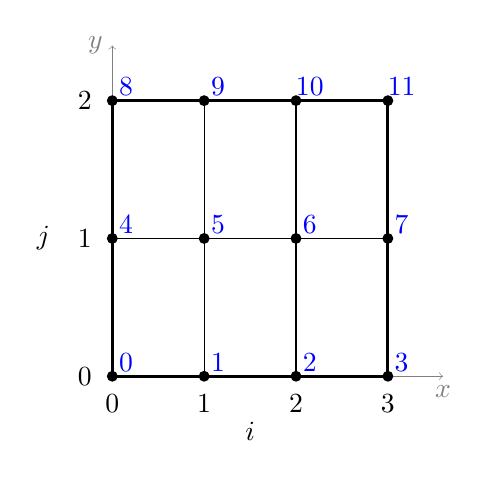
\begin{tikzpicture}[scale=3.5]
  \draw[->,gray,very thin] (0.0,0.0) -- (1.2,0.0) node[below] {$x$};
  \draw[->,gray,very thin] (0.0,0.0) -- (0.0,1.2) node[left] {$y$};
  \draw[line width=1.0pt] (0.0,0.0) -- (0.0,1.0) -- (1.0,1.0) -- (1.0,0.0) -- cycle;
  \pgfmathsetmacro\third{1.0/3.0}
  \pgfmathsetmacro\half{1.0/2.0}
  \node at (0.0,-0.1) {$0$};
  \node at (\third,-0.1) {$1$};
  \node at (\half,-0.2) {$i$};
  \node at (2*\third,-0.1) {$2$};
  \node at (1.0,-0.1) {$3$};
  \node at (-0.1,0.0) {$0$};
  \node at (-0.1,0.5) {$1$};
  \node at (-0.25,0.5) {$j$};
  \node at (-0.1,1.0) {$2$};
  \draw[xstep=\third,ystep=\half,black,thin] (0.0,0.0) grid (1.0,1.0);
  \pgfmathsetmacro\dd{0.05}
  \foreach \y in {0,1,2}
    \foreach \x in {0,1,2,3} {
      \pgfmathsetmacro\k{4*\y+\x}
      \draw[color=blue] (\x*\third+\dd,\y*\half+\dd) node{\pgfmathprintnumber[fixed]{\k}};
      \filldraw (\x * \third,\y * \half) circle (0.5pt);
    }
\end{tikzpicture}
\caption{Ordering of unknowns \eqref{orderingfd} on a $M=4$ and $N=3$ grid.  Index $k = j\,M + i$ is shown in {\color{blue} blue}.}
\label{fig:unitsquaregridordering}
\end{marginfigure}

\medskip\noindent\hrulefill
\begin{example} In the $M=4$ and $N=3$ case shown in Figure \ref{fig:unitsquaregridordering} we have grid spacing $h_x=1/3$ and $h_y=1/2$.  Equations \eqref{poissonsquareFDearly} and \eqref{poissonsquareFDbcs} are an invertible system of $K=12$ equations.  Only the $k=5$ and $k=6$ equations are not boundary conditions \eqref{poissonsquareFDbcs}.  Thus the linear system is
\setcounter{MaxMatrixCols}{20}
\begin{equation*}
\begin{bmatrix}
1 &  &  &  &  &  &  &  &  &  &  &  \\
  & 1&  &  &  &  &  &  &  &  &  &  \\
  &  & 1&  &  &  &  &  &  &  &  &  \\
  &  &  & 1&  &  &  &  &  &  &  &  \\
  &  &  &  & 1&  &  &  &  &  &  &  \\
  & c&  &  & b& a& b&  &  & c&  &  \\
  &  & c&  &  & b& a& b&  &  & c&  \\
  &  &  &  &  &  &  & 1&  &  &  &  \\
  &  &  &  &  &  &  &  & 1&  &  &  \\
  &  &  &  &  &  &  &  &  & 1&  &  \\
  &  &  &  &  &  &  &  &  &  & 1&  \\
  &  &  &  &  &  &  &  &  &  &  & 1
\end{bmatrix}
\begin{bmatrix}
U_{0,0} \\
U_{1,0} \\
U_{2,0} \\
U_{3,0} \\
U_{0,1} \\
U_{1,1} \\
U_{2,1} \\
U_{3,1} \\
U_{0,2} \\
U_{1,2} \\
U_{2,2} \\
U_{3,2}
\end{bmatrix}
=
\begin{bmatrix}
0 \\
0 \\
0 \\
0 \\
0 \\
f_{1,1} \\
f_{2,1} \\
0 \\
0 \\
0 \\
0 \\
0
\end{bmatrix}
\end{equation*}
where $a = 2/h_x^2 + 2/h_y^2 = 26$, $b = - 1/h_x^2 = -9$ and $c = - 1/h_y^2 = -4$.

Note that the matrix $A$ is not symmetric.  Furthermore it is not well-scaled for such a small example.  For instance, its 2-norm condition number \citep{TrefethenBau} is $\cond(A) = \|A\|_2 \|A^{-1}\|_2 = 43.16$.
\end{example}
\noindent\hrulefill

Before assembling the system by writing \PETSc code, there are two nontrivial observations about it.  First, the equations \eqref{poissonsquareFDearly} have very different ``scaling'' from those in \eqref{poissonsquareFDbcs}.  For example, if $M=N=1001$, so that $h_x=h_y=0.001$, then the coefficient of $U_{i,j}$ in \eqref{poissonsquareFDearly} is $4/(.001)^2 = 4 \times 10^6$, while the coefficients along the boundary, from equations \eqref{poissonsquareFDbcs}, are equal to 1.

\begin{marginfigure}
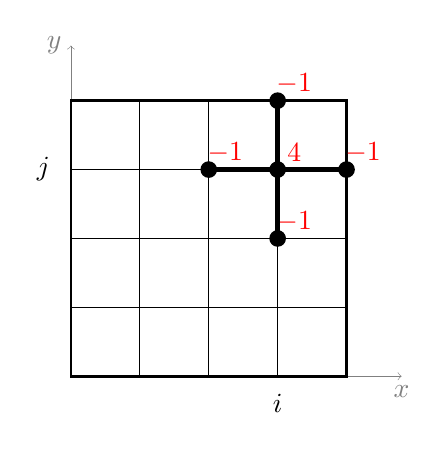
\begin{tikzpicture}[scale=3.5]
  \draw[->,gray,very thin] (0.0,0.0) -- (1.2,0.0) node[below] {$x$};
  \draw[->,gray,very thin] (0.0,0.0) -- (0.0,1.2) node[left] {$y$};
  \draw[line width=1.0pt] (0.0,0.0) -- (0.0,1.0) -- (1.0,1.0) -- (1.0,0.0) -- cycle;
  \node at (0.75,-0.1) {$i$};
  \node at (-0.1,0.75) {$j$};
  \filldraw (0.50,0.75) circle (0.8pt);
  \filldraw (0.75,0.75) circle (0.8pt);
  \filldraw (1.00,0.75) circle (0.8pt);
  \filldraw (0.75,0.5) circle (0.8pt);
  \filldraw (0.75,1.0) circle (0.8pt);
  \pgfmathsetmacro\dd{0.06}
  \draw[color=red] (0.75+\dd,0.75+\dd) node{$4$};
  \draw[color=red] (0.5+\dd,0.75+\dd)  node{$-1$};
  \draw[color=red] (0.75+\dd,0.5+\dd)  node{$-1$};
  \draw[color=red] (1.0+\dd,0.75+\dd)  node{$-1$};
  \draw[color=red] (0.75+\dd,1.0+\dd)  node{$-1$};
  \draw[line width=2.0pt] (0.50,0.75) -- (1.00,0.75);
  \draw[line width=2.0pt] (0.75,0.5)  -- (0.75,1.00);
  \draw[xstep=0.25,ystep=0.25,black,thin] (0.0,0.0) grid (1.0,1.0);
\end{tikzpicture}
\caption{For a grid with equal spacing $h_x=h_y$, the coefficients on the left side of \eqref{poissonsquareFD}, as shown here in {\color{red} red}, are the well-known ``$4$'' and ``$-1$'' for the stencil of the Laplacian.}
\label{fig:equalstarstencil}
\end{marginfigure}

Thus, to make the equations better scaled, and also to match the scaling that is automatic in the finite element method (see Chapter 3), we multiply equation \eqref{poissonsquareFDearly} by the grid cell area $h_x h_y$ to get
\begin{align}
&\left(2 \frac{h_y}{h_x} + 2 \frac{h_x}{h_y}\right) U_{i,j} - \frac{h_y}{h_x}\left(U_{i+1,j} + U_{i-1,j}\right)  - \frac{h_x}{h_y}\left(U_{i,j+1} + U_{i,j-1}\right) \label{poissonsquareFD} \\
&\qquad = h_x h_y f_{i,j}. \notag
\end{align}
Using \eqref{poissonsquareFD}, as long as the cell aspect ratio $\max\{h_y/h_x,h_x/h_y\}$ is not too large, all the equations in the system, including the boundary conditions, will have coefficients of comparable size.  If $h_x=h_y$ then the diagonal entries are equal to $4$ and the off-diagonal entries are $-1$; see the well-known stencil in Figure \ref{fig:equalstarstencil}.

Our second nontrivial observation is that our equations can be re-interpreted to give a \emph{symmetric} matrix $A$.  This opens up a larger range of linear algebra methods for solving the system efficiently.  For example, in the $i=1$ case of \eqref{poissonsquareFD}, i.e.~at a grid point adjacent to the left-hand boundary of the square, the boundary location value $U_{0,j}$ appears in the equation.  The matrix in the linear system will be symmetric if we systematically ``move'' such values to the right-hand side as known (and zero), instead of inserting a ``$1$'' into the corresponding matrix locations.  That is, we force off-diagonal entries to be zero in those columns corresponding to known boundary values, in addition to the off-diagonal zeros in the boundary-value rows.

With these two modifications we can redo the previous $M=4$ and $N=3$ example.

\medskip\noindent\hrulefill
\begin{example} For the same $M=4$ and $N=3$ case shown in Figure \ref{fig:unitsquaregridordering}, equations \eqref{poissonsquareFDbcs} and \eqref{poissonsquareFD} become
\begin{equation*}
\begin{bmatrix}
1 &  &  &  &  &  &  &  &  &  &  &  \\
  & 1&  &  &  &  &  &  &  &  &  &  \\
  &  & 1&  &  &  &  &  &  &  &  &  \\
  &  &  & 1&  &  &  &  &  &  &  &  \\
  &  &  &  & 1&  &  &  &  &  &  &  \\
  &  &  &  &  & \alpha& \beta&  &  &  &  &  \\
  &  &  &  &  & \beta& \alpha&  &  &  &  &  \\
  &  &  &  &  &  &  & 1&  &  &  &  \\
  &  &  &  &  &  &  &  & 1&  &  &  \\
  &  &  &  &  &  &  &  &  & 1&  &  \\
  &  &  &  &  &  &  &  &  &  & 1&  \\
  &  &  &  &  &  &  &  &  &  &  & 1
\end{bmatrix}
\begin{bmatrix}
U_{0,0} \\
U_{1,0} \\
U_{2,0} \\
U_{3,0} \\
U_{0,1} \\
U_{1,1} \\
U_{2,1} \\
U_{3,1} \\
U_{0,2} \\
U_{1,2} \\
U_{2,2} \\
U_{3,2}
\end{bmatrix}
=
\begin{bmatrix}
0 \\
0 \\
0 \\
0 \\
0 \\
(1/6) f_{1,1} \\
(1/6) f_{2,1} \\
0 \\
0 \\
0 \\
0 \\
0
\end{bmatrix}
\end{equation*}
where $\alpha = 2 (h_y/h_x) + 2 (h_x/h_y) = 13/3$ and $\beta = - h_y/h_x = - 3/2$.  The matrix is both symmetric and better-scaled, with $\cond(A)=5.83$.
\end{example}
\noindent\hrulefill

We now present the core code, in Figure \ref{code:structuredlaplacian}, that assembles ``$A$'' in our linear system \eqref{poissonlinearsystem}.  For clarity and code reuse we have isolated method \texttt{formdirichletlaplacian()} in a separate file; we will use it both to solve the Poisson and the heat equations below.

\begin{marginfigure}
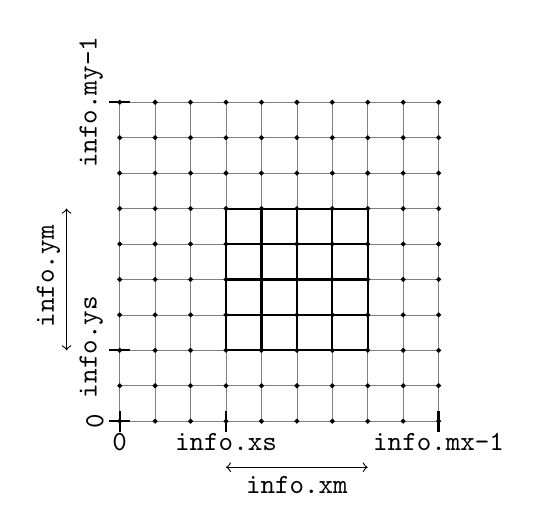
\begin{tikzpicture}[scale=4.5]
  % global grid, local grid, nodes
  \draw[xstep=0.1,ystep=0.1,gray,very thin] (0.0,0.0) grid (0.9,0.9);
  \draw[xstep=0.1,ystep=0.1,black,thick] (0.3,0.2) grid (0.7,0.6);
  \foreach \y in {0,...,9}
    \foreach \x in {0,...,9} {
      \filldraw (\x * 0.1,\y * 0.1) circle (0.15pt);
    }
  % ticks on x-axis at 0, xs, mx
  \draw[black,thick] (0,-0.03)   -- (0,+0.03);
  \draw[black,thick] (0.3,-0.03) -- (0.3,+0.03);
  \draw[black,thick] (0.9,-0.03) -- (0.9,+0.03);
  \node at (0,-0.06) {\texttt{0}};
  \node at (0.3,-0.06) {\texttt{info.xs}};
  \node at (0.9,-0.06) {\texttt{info.mx-1}};
  % ticks on y-axis at 0, ys, my
  \draw[black,thick] (-0.03,0)   -- (+0.03,0);
  \draw[black,thick] (-0.03,0.2) -- (+0.03,0.2);
  \draw[black,thick] (-0.03,0.9) -- (+0.03,0.9);
  \node[rotate around={90:(0,0)}] at (-0.07,0) {\texttt{0}};
  \node[rotate around={90:(-0.2,0.2)}] at (-0.08,0.12) {\texttt{info.ys}};
  \node[rotate around={90:(0.0,0.9)}] at (-0.28,0.7) {\texttt{info.my-1}};
  % xm, ym along sides of local patch
  \draw[<->,] (0.3,-0.13) -- (0.7,-0.13);
  \node at (0.5,-0.18) {\texttt{info.xm}};
  \draw[<->,] (-0.15,0.2) -- (-0.15,0.6);
  \node[rotate around={90:(0.3-0.3,0.4)}] at (-0.29,0.32) {\texttt{info.ym}};
\end{tikzpicture}
\caption{How \texttt{DMDALocalInfo info} describes the indices for your local process' part of the grid.}
\label{fig:localpartofgrid}
\end{marginfigure}

Its first action is to extract from the \pDM object \texttt{da} a variable \texttt{info} of type \texttt{DMDALocalInfo}.  In particular, this object has the global grid size in members \texttt{info.mx,info.my} so we can compute grid spacings \texttt{hx,hy}.  Significantly, \texttt{info} can tell us the part of the grid owned by the local processor.  The local process has a \texttt{info.xm} by \texttt{info.ym} rectangular subgrid, with a range of indices
   $$\text{\texttt{info.xs}} \le i \le \text{\texttt{info.xs}} +\text{\texttt{info.xm}}$$
and
   $$\text{\texttt{info.ys}} \le j \le \text{\texttt{info.ys}} +\text{\texttt{info.ym}}.$$
See Figure \ref{fig:localpartofgrid}.


For example, in Figure \ref{fig:unitsquaregridparallel} the rank $0$ process has \text{\texttt{info.xs}}$=0$ and \text{\texttt{info.xm}}$=3$ while the rank $1$ process has \text{\texttt{info.xs}}$=3$ and \text{\texttt{info.xm}}$=2$.  Such index ranges are reflected in \texttt{for} loops which re-appear every time we do operations on a structured 2D grid:
\begin{Verbatim}[fontsize=\small]
  for (j=info.ys; j<info.ys+info.ym; j++) {
    for (i=info.xs; i<info.xs+info.xm; i++) {
      DO SOMETHING AT GRID POINT (i,j)
    }
  }
\end{Verbatim}

\cinput{structuredlaplacian.c}{Fill matrix entries using \texttt{MatSetValuesStencil}.}{//CREATEMATRIX}{//ENDCREATEMATRIX}{code:structuredlaplacian}

The \pMat object we assemble has ranges of rows owned by each process.  But we don't need to know that on a \pDMDA-managed structured grid.  Instead we work though our locally-owned part of the grid and we use the $(i,j)$ description of a point and its stencil neighbors to insert entries into a dynamical data structure which is a non-yet-assembled \pMat.  That is, in Figure \ref{code:structuredlaplacian} we see one command \texttt{MatSetValuesStencil()} for each locally-owned grid point, and for the generic interior point that \texttt{MatSetValuesStencil()} command inserts five coefficients into the matrix.  The key data structure is of type \texttt{MatStencil}, which is an apparently trivial struct
\begin{Verbatim}[fontsize=\small]
typedef struct {
  PetscInt k,j,i,c;
} MatStencil;
\end{Verbatim}
In our 2D case, with a single degree of freedom at each node,\sidenote{That is, Poisson problem \eqref{poissonsquare} is a scalar PDE so the unknown at each grid point is the scalar $U_{i,j}$.  A system of equations like Maxwell's or Navier-Stokes would have \texttt{dof}$>1$ when we call \texttt{DMDACreateXd()}.} we only use the \texttt{i} and \texttt{j} members of \texttt{MatStencil}.

From \eqref{poissonsquareFD}, the actual matrix entries are either $a_{i,i} = 2\left(h_y/h_x + h_x/h_y\right)$ on the diagonal and either $a_{i,j} = -h_y/h_x$ or $a_{i,j} = -h_x/h_y$ if an off-diagonal entry is nonzero.  Furthermore, as mentioned above, we only insert nonzeros in the matrix if the corresponding column in the matrix is a non-boundary location.

After completing all the \texttt{MatSetValuesStencil()} commands we call 
\begin{Verbatim}[fontsize=\small]
  MatAssemblyBegin(A,MAT_FINAL_ASSEMBLY);
  MatAssemblyEnd(A,MAT_FINAL_ASSEMBLY);
\end{Verbatim}
just as we did in Chapter 1.

\cinputpart{c2poisson.c}{The right side of equation \eqref{poissonsquareFD} comes from differentiating the exact solution, which this method also computes.}{I}{//RHS}{//ENDRHS}{code:ctwopoissonrhs}

\cinputpart{c2poisson.c}{Set up \pDMDA \texttt{da} and \pMat \texttt{A} objects, and assemble the latter by calling \texttt{formlaplacian()}.}{II}{//CREATE}{//ENDCREATE}{code:ctwopoissoncreate}

\cinputpart{c2poisson.c}{Solve using \pKSP, and report on solution.}{III}{//SOLVE}{//ENDSOLVE}{code:ctwopoissonsolve}

\section{Runtime control of linear solver}

FIXME: basic Krylov theory

\section{Time-dependent heat equation}

FIXME: we WON'T do explicit, but it would look like ...

FIXME: use TS for backward-euler
